\newpage
\section{Eksisterende løsninger}
I dette afsnit vil de nuværende IT-løsninger, som har indvirken på problematikker vedrørende o-løbstræning, blive forklaret og analyseret. 

\subsection{Endomondo}
Endomondo er en applikation som bruges til løb, hvori en træningsplan kan udformes. Applikationen vil her have to versioner, en gratis og en udvidelses-version som kan købes. Endomondo bruger Google Maps som kort i deres applikation \citep{ENDOMAPS}. Funktionaliteten der her vil blive beskrevet er for gratis versionen: Hovedmenu med otte funktioner:
\begin{itemize}
	\item Newsfeed, som bruges til at kommunikere med andre brugere af Endomondo, hvor brugere kan opmuntre, samt udfordre hinanden til løb og andre udfordringer.
	\item Notifikationer, hvor brugeren kan se sine udfordringer og lignende fra andre brugere. Her kan brugeren acceptere eller afslå udfordringer.
	\item Historik, hvor tidligere løb oplagres til genvisning og statistik.
	\item Kort, hvor brugeren ved hjælp af mobilens GPS-enhed kan få et kort over ruten der er løbet.
	\item Opgrader-nu, hvor gratis versionen kan betales til opgradering.
	\item Venner, hvor brugeren kan overvære venner fra sociale medier.
	\item Træningsplanen, der bruges til at indstille applikationens hjælpefunktioner til træning, hvor brugeren selv sætter mål for træningen, intensiteten ved træningen, og hvilken type af træning der udøves.
	\item Indstillinger, hvor de generelle indstillinger for programmet kan tilpasses.
\end{itemize}
Dette er en velfungerende applikation til formålet, løb og træningsplan, men i det at en o-løber skal bruge visningen af løbet på et o-løbskort, kan dette blive problematisk, da brugeren ikke selv kan sætte kort ind i programmet. 


\subsection{EMIT brikker}
\begin{wrapfigure}{r}{0.5\textwidth}
	\vspace{5pt}
	\begin{center}
		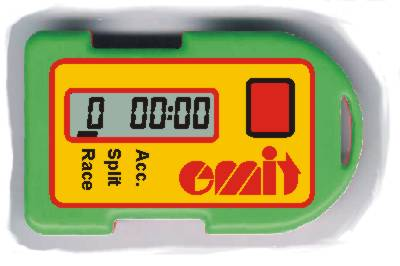
\includegraphics[width=0.4\textwidth]{billeder/emitbrik}
	\end{center}
	\vspace{-20pt}
	\caption{EMIT brik}
	\vspace{-10pt}
\end{wrapfigure}
En EMIT brik, er et elektronisk apparat, der kan registrere hvilke poster der besøges. EMIT brikken sidder fast på fingeren, vha. en elastik. Et billede af EMIT brikken kan ses på figur 2.3.

Måden en EMIT brik fungere på, er at den stilles på en startpost ca. 5 sekunder før løbet bliver sat i gang. Dette vil genstarte EMIT brikken, således at den kan notere de rigtige tider. 
Ved hver post, der skal besøges, er der en kontrolpost, der ligner startposten, som EMIT brikken skal lægges på i ca. ½ sekund. Dette vil registrere hvor lang tid der er gået mellem forrige post og nuværende post. \newline
Til sidst i løbet, vil der være en målpost, hvor EMIT brikken endnu engang skal lægges på, således at den sidste tid bliver noteret. 
Herefter skal EMIT brikken afleveres til de ansvarlige, som vil give løberen en udskrift af tiderne. Disse tider kan så derefter anvendes til sammenligning og diskussion med andre løbere. \citep{OOK}

\subsection{QuickRoute}
Igennem gruppens interview, beskrev Claus, at QuickRoute er en eksisterende løsning til kortlæggelse og rutevisning. For at bruge denne løsning skal løberen have et Garmin ur, eller andre GPS enheder, som kan generere en GPX fil over ruten. I QuickRoute kan et kort fra OCAD (OCAD er et program til at lave o-løbskort) lægges ind, og ved hjælp af Garmin ure kan en rute blive vist, hvor forskellige parametre kan blive afbildet. Hastighed, minutter per kilometer, hjertefrekvens, højdemeter og afvigelse fra retningen mellem to punkter kan blive afbildet. Dette bliver vist ved en farvekode der følger ruten, og gennem hele ruten vil denne farvekode variere efter hvert interval af GPS-signal. Med den rigtige serie af Garmin ure, kan der tilmed tages tid på, hvornår en post er nået, så en statistisk model kan beskrive tiderne mellem posterne. Hvis musen holdes over et punkt på ruten, kan følgende information om punktet vises: Klokkeslæt, tid brugt i alt på rute, samlet distance løbet til det punkt, nuværende minutter per kilometer, nuværende hastighed i km/t, nuværende hjertefrekvens, nuværende højdemeter, nuværende afvigelse mellem to punkter, nuværende længde- og breddegrader. Mange af disse informationer kan afbildes på et histogram. \citep{QR}

\begin{figure}[h]
	\centering
	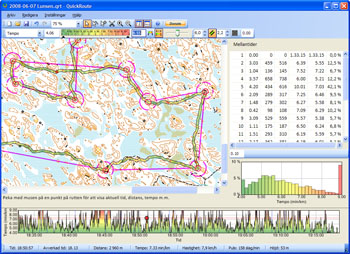
\includegraphics[width=0.8\textwidth]{billeder/QR}
	\caption{Screenshot af QuickRoute}
\end{figure}

Derudover kan ruten efterfølgende integreres på Google Earth, så der kan ses en 3D model af ruten der er løbet. 
Denne løsning er meget gennemført, hvor mange funktioner kan benyttes, dog kan antallet af funktioner og parametre virke overflødig for en amatør o-løber. For en rutineret eller professionel o-løber vil denne løsning give et godt indblik i, hvordan løbet er foregået og hvor personen kan udvikle sig. QuickRoute kan også bruges til sammenligning mellem løbere, dette kræver dog at begge løbere GPX-filer bliver lagt over på samme computer, og loaded ind i programmet. 


\subsection{TracTrac}
TracTrac er en samlet løsning til livetracking med replay funktion af forskellige sport events. Til dette bruges TracTrac's egne GPS enheder. Disse er ca. på størrelse med en cigaretpakke og vejer 113 gram.\newline
TracTrac bruges til o-løb så der live kan følges med i hvor o-løberne er ude i terrænet, som f. eks. til stævner og konkurrencer. Derudover bruges TracTrac i høj grad til at analysere de enkelte løberes ture efter de har løbet, da TracTrac har en velfungerende replay funktion. 

Når TracTrac skal bruges i forbindelse med o-løb, laves der først et o-løbskort som uploades til TracTracs servere. Derefter indsættes præcise punkter på kortet som repræsentere hvor hver enkelt post ligger, så TracTrac kender positionerne på alle posterne. Herefter skal hver enkelt GPS enhedsnummer sættes sammen med en løber, så det bliver tydeligt hvem der løber hvor. Under løbet sender GPS enhederne deres position til serverne som viser disse på kortet. Alt dette sker live. En af funktionerne som gør TracTrac ekstra brugbar i forbindelse med o-løb, er dens mulighed for at flytte løbere tilbage til start og afspille deres tur samtidig, så der kan ses præcist hvordan de løb i forhold til hinanden, selvom de i virkeligheden startede forskudt. Dette kan også gøres selvom løbet er live. En løber der er foran, kan flyttes tilbage, så vedkommende løber samtidig, som en anden løber der er startet senere. Dette giver mulighed for grundig analyse og sammenligning af løbernes vejvalg og hastighed, både under og efter løbet.\newline
TracTrac kan stort set alt der er brug for til live visning og analyse af o-løb. Selve GPS-enheden koster 150 EUR, altså lige godt 1120 DKK. Derudover skal der bruges et sim, data kort og enhedslicens til 88 EUR om året pr. enhed, hvilket vil svare til ca. 650 DKK. Som det sidste skal en system-licens bruges, denne koster 990 EUR årligt, hvilket er ca. 7380 DKK. Dette produkt er i sådan en prisklasse, at de små amatørklubber ikke har råd til det. \citep{TTC}


\subsubsection{Opsummering}
Ud fra ovenstående analyse af eksisterende løsninger, kan det konkluderes, at der findes metoder der kan hjælpe o-løbere med at optimere deres træning. I form af QuickRoute, er der mulighed for at analysere de forskellige ruter løberen har kunnet vælge imellem, samtidig sammenligne med andre løbere. Dette kræver dog at løberne har en GPS tracker, som et Garmin ur, hvilket gør en sammenligning vanskelig. TracTrac giver mulighed for at det kan følges live, og dermed er der også mulighed for at se replay af løbeturen, herudover kan der også sammenlignes med tal ud fra ruterne. Denne løsning kræver dog ikke Garmin ure, men kræver nogle TracTrac enheder, og noget licens, der hurtigt kan blive for dyrt, for de mindre foreninger og derfor ikke helt optimalt. 
Gruppen vurderer derfor, at en mulig løsning på dette, er anvendelse af mobiltelefoner som GPS enhed. En mobiltelefon er let tilgængelig, og der er mulighed for GPS tracking på den, og der behøves ikke ekstra omkostninger, som fx. ved et Garmin ur eller TracTrac licens. Endomondo bruger mobilens GPS signal, men da der ikke en nogen replay funktion eller mulighed for at lægge andet end Google Maps' kort bag ruten, er denne løsning ikke velegnet til o-løb. 